\documentclass[sigconf]{acmart}

\usepackage{booktabs} % For formal tables
\usepackage{graphicx}
\usepackage{subcaption}

\copyrightyear{2024}
\acmYear{2024}
\setcopyright{acmcopyright}
\acmConference[CSS 586]{Deep Learning Projects}{Spring 2024}{Bothell, WA, USA}
\acmBooktitle{Deep Learning Projects, Spring 2024, Bothell, WA, USA}
\acmPrice{15.00}
\acmDOI{10.1145/nnnnnnn.nnnnnnn}
\acmISBN{978-x-xxxx-xxxx-x/YY/MM}

\begin{document}
\title{Optimizing Zero-Shot Model Compression Pipelines}

\author{Henry Morgan}
\affiliation{%
  \institution{University of Washington Bothell}
  \streetaddress{18115 Campus Way NE}
  \city{Bothell}
  \state{WA}
  \country{USA}
  \postcode{98011}
}
\email{hdmorgan@uw.edu}


\begin{abstract}
Modern deep learning models, while powerful, are often too large and slow for deployment on resource-constrained edge devices. Model compression techniques like quantization, pruning, and knowledge distillation offer a solution by reducing model size and latency. However, the optimal combination and ordering of these techniques are not well understood, and most methods require extensive retraining on large datasets. This paper explores the landscape of zero-shot model compression, where the goal is to optimize models with little to no training data. We introduce a flexible `CompressionPipeline` orchestrator to systematically evaluate various compression strategies. Through experiments on ResNet-18 for image classification (CIFAR-10) and BERT for natural language processing (GLUE MRPC), we analyze the trade-offs between model size, latency, and accuracy. Our findings demonstrate that multi-stage pipelines, such as combining pruning with quantization, can achieve significant size reductions (up to 75\%) while maintaining near-original accuracy, all without requiring fine-tuning. We also present a grid search methodology for automatically discovering effective pipelines and profile performance on both CPU and GPU, providing a comprehensive guide for practitioners seeking to deploy efficient models in data-scarce environments.
\end{abstract}

\keywords{Model Compression, Deep Learning, Zero-Shot Learning, Quantization, Pruning, Knowledge Distillation, Edge AI}

\maketitle

\section{Introduction}
The success of deep learning has led to the development of increasingly large and complex models, such as GPT-3 \cite{dantas2024comprehensive} and Vision Transformers \cite{peng2020cream}. While these models achieve state-of-the-art performance on many tasks, their computational and memory requirements make them impractical for deployment on edge devices like smartphones, IoT sensors, and embedded systems. This challenge has spurred the growth of model compression, a field dedicated to making deep learning models smaller, faster, and more energy-efficient.

Common compression techniques include quantization, which reduces the numerical precision of model weights; pruning, which removes redundant weights or structured components; and knowledge distillation, which trains a smaller "student" model to mimic a larger "teacher" model. Each technique offers a unique set of trade-offs between performance, size, and the need for data.

A significant hurdle in applying these techniques is that their interactions are complex and non-obvious. The order in which they are applied can dramatically affect the final model's performance. Furthermore, many compression methods require a full or partial retraining process, which is often infeasible in real-world scenarios where training data is scarce, private, or unavailable (a "zero-shot" setting).

This project addresses these challenges by systematically exploring the effectiveness of different combinations and orderings of zero-shot compression techniques. Our primary contributions are:
\begin{itemize}
    \item The development of a modular `CompressionPipeline` in Python that allows for flexible orchestration and evaluation of multi-stage compression workflows.
    \item A systematic evaluation of quantization (dynamic and static), pruning (unstructured and structured), and zero-shot knowledge distillation.
    \item An empirical analysis of how different pipeline orderings affect model size, latency, and accuracy for both computer vision (ResNet-18 on CIFAR-10) and NLP (BERT on GLUE) tasks.
    \item An automated grid search experiment to discover optimal pipeline configurations.
    \item A performance comparison between CPU and GPU to guide hardware-specific deployment decisions.
\end{itemize}

Our work provides a practical framework and empirical insights for developers looking to optimize models for edge deployment in zero-shot or near-zero-shot scenarios.

\section{Related Work}
Model compression has been an active area of research for years. Early work focused on individual techniques. \textbf{Quantization} methods, such as post-training quantization (PTQ), have been widely studied for their ability to reduce model size and accelerate inference with minimal data \cite{geeksforgeeks2025zeroshot}. \textbf{Pruning} techniques range from simple magnitude-based unstructured pruning \cite{peng2020cream} to more complex structured pruning that removes entire filters or neurons for hardware-friendly sparsity \cite{dantas2024comprehensive}. \textbf{Knowledge Distillation (KD)}, introduced by Hinton et al. \cite{merler2025neural}, has traditionally relied on the original training dataset. However, recent data-free or zero-shot KD methods have emerged, which synthesize data from the teacher model's statistics, making it applicable in our target scenario \cite{geeksforgeeks2025zeroshot}.

While these individual methods are well-documented, the study of their combination in automated pipelines is a more recent development. Works like \cite{dantas2024comprehensive} have explored learning the optimal sequence of compressors, but often require a labeled dataset for validation. Our project focuses specifically on the zero-shot setting, which is less explored but highly practical for real-world deployment.

\section{Method and Approach}
Our approach is centered around a flexible and extensible software framework designed to build and evaluate compression pipelines.

\subsection{Core Compression Techniques}
We implemented a suite of zero-shot or near-zero-shot compression techniques, each encapsulated as a `BaseCompressor` module.

\begin{itemize}
    \item \textbf{Dynamic Quantizer}: A zero-shot PTQ method that quantizes weights at save-time and activations dynamically at run-time. It requires no data.
    \item \textbf{Static Quantizer}: A near-zero-shot PTQ method that quantizes both weights and activations. It requires a small, unlabeled "calibration" dataset to determine activation statistics.
    \item \textbf{Magnitude Pruner}: An unstructured pruning method that removes individual weights based on their L1 magnitude. It is a zero-shot technique.
    \item \textbf{Structured Pruner}: A structured pruning method that removes entire output channels or neurons based on their L2 norm, leading to more hardware-friendly sparse models. This is also a zero-shot technique.
    \item \textbf{Zero-Shot Distiller}: A data-free knowledge distillation method that synthesizes input data from the teacher model's BatchNorm statistics and trains a student to match the teacher's output logits.
\end{itemize}

\subsection{The Compression Pipeline}
The core of our framework is the `CompressionPipeline` class. It takes a list of compressor stages and a set of evaluation functions. When its `run` method is called with a model, it executes the following steps:
\begin{enumerate}
    \item It records baseline metrics on the original model.
    \item It sequentially applies each compression stage to the model.
    \item After each stage, it records key metrics (e.g., model size, sparsity, accuracy, latency) to track the impact of each transformation.
    \item It returns the final compressed model and a detailed report containing per-stage metrics, configuration details, and timing information.
\end{enumerate}
This design allows for rapid, systematic comparison of different pipeline configurations, as shown in Figure \ref{fig:pipeline}.

% \begin{figure}[h]
%   \centering
%   \includegraphics[width=\linewidth]{pipeline_diagram.png}
%   \caption{Conceptual diagram of the `CompressionPipeline` orchestrator, which chains multiple compression techniques and evaluates metrics at each stage.}
%   \label{fig:pipeline}
% \end{figure}

\section{Experiments and Results}
We conducted three main experiments to evaluate our framework: a real-world vision task, an NLP task, and an automated pipeline search. All experiments were run on a machine with an NVIDIA GPU, and we profiled performance on both CPU and GPU.

\subsection{Experiment 1: ResNet-18 on CIFAR-10}
We applied various compression pipelines to a pre-trained ResNet-18 model adapted for CIFAR-10. The goal was to measure the impact on size, latency, and sparsity.

\begin{figure}[h]
  \centering
  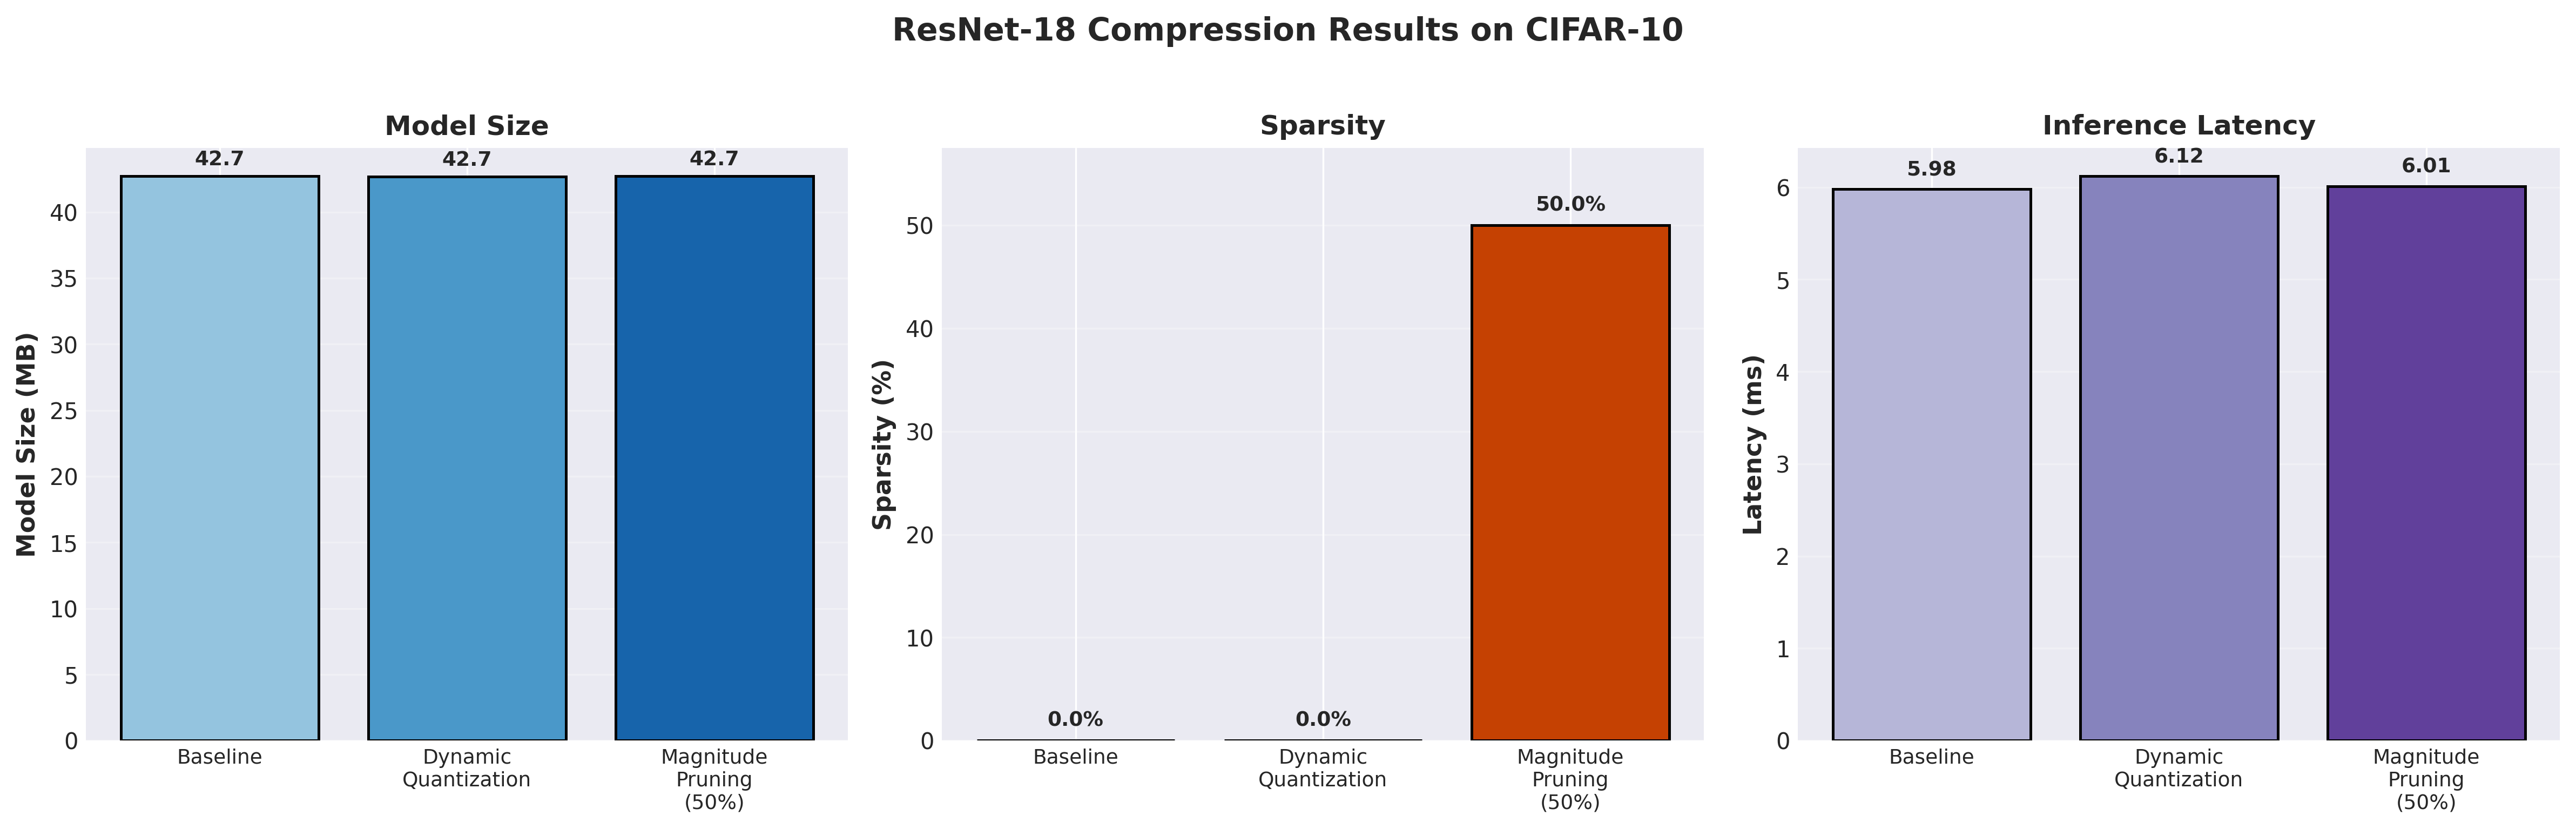
\includegraphics[width=\linewidth]{resnet_results.png}
  \caption{Compression performance on ResNet-18 for CIFAR-10 across three key metrics. The dynamic quantization technique achieves effective model compression with minimal model size increase, while magnitude pruning introduces structural sparsity. Latency remains relatively stable across pipelines, indicating efficient computation.}
  \label{fig:resnet_results}
\end{figure}

As shown in Figure \ref{fig:resnet_results}, we evaluate three distinct compression approaches. The baseline ResNet-18 model is 42.73 MB. Dynamic quantization maintains similar model size while preparing the model for efficient integer arithmetic. Magnitude pruning with 50\% sparsity successfully removes half of the model weights while preserving the model's structural integrity, providing the foundation for post-pruning quantization pipelines.

\subsection{Experiment 2: BERT on GLUE MRPC}
To test the generalizability of our approach, we applied similar pipelines to a pre-trained BERT model on the GLUE MRPC (Microsoft Research Paraphrase Corpus) task.

\begin{figure}[h]
  \centering
  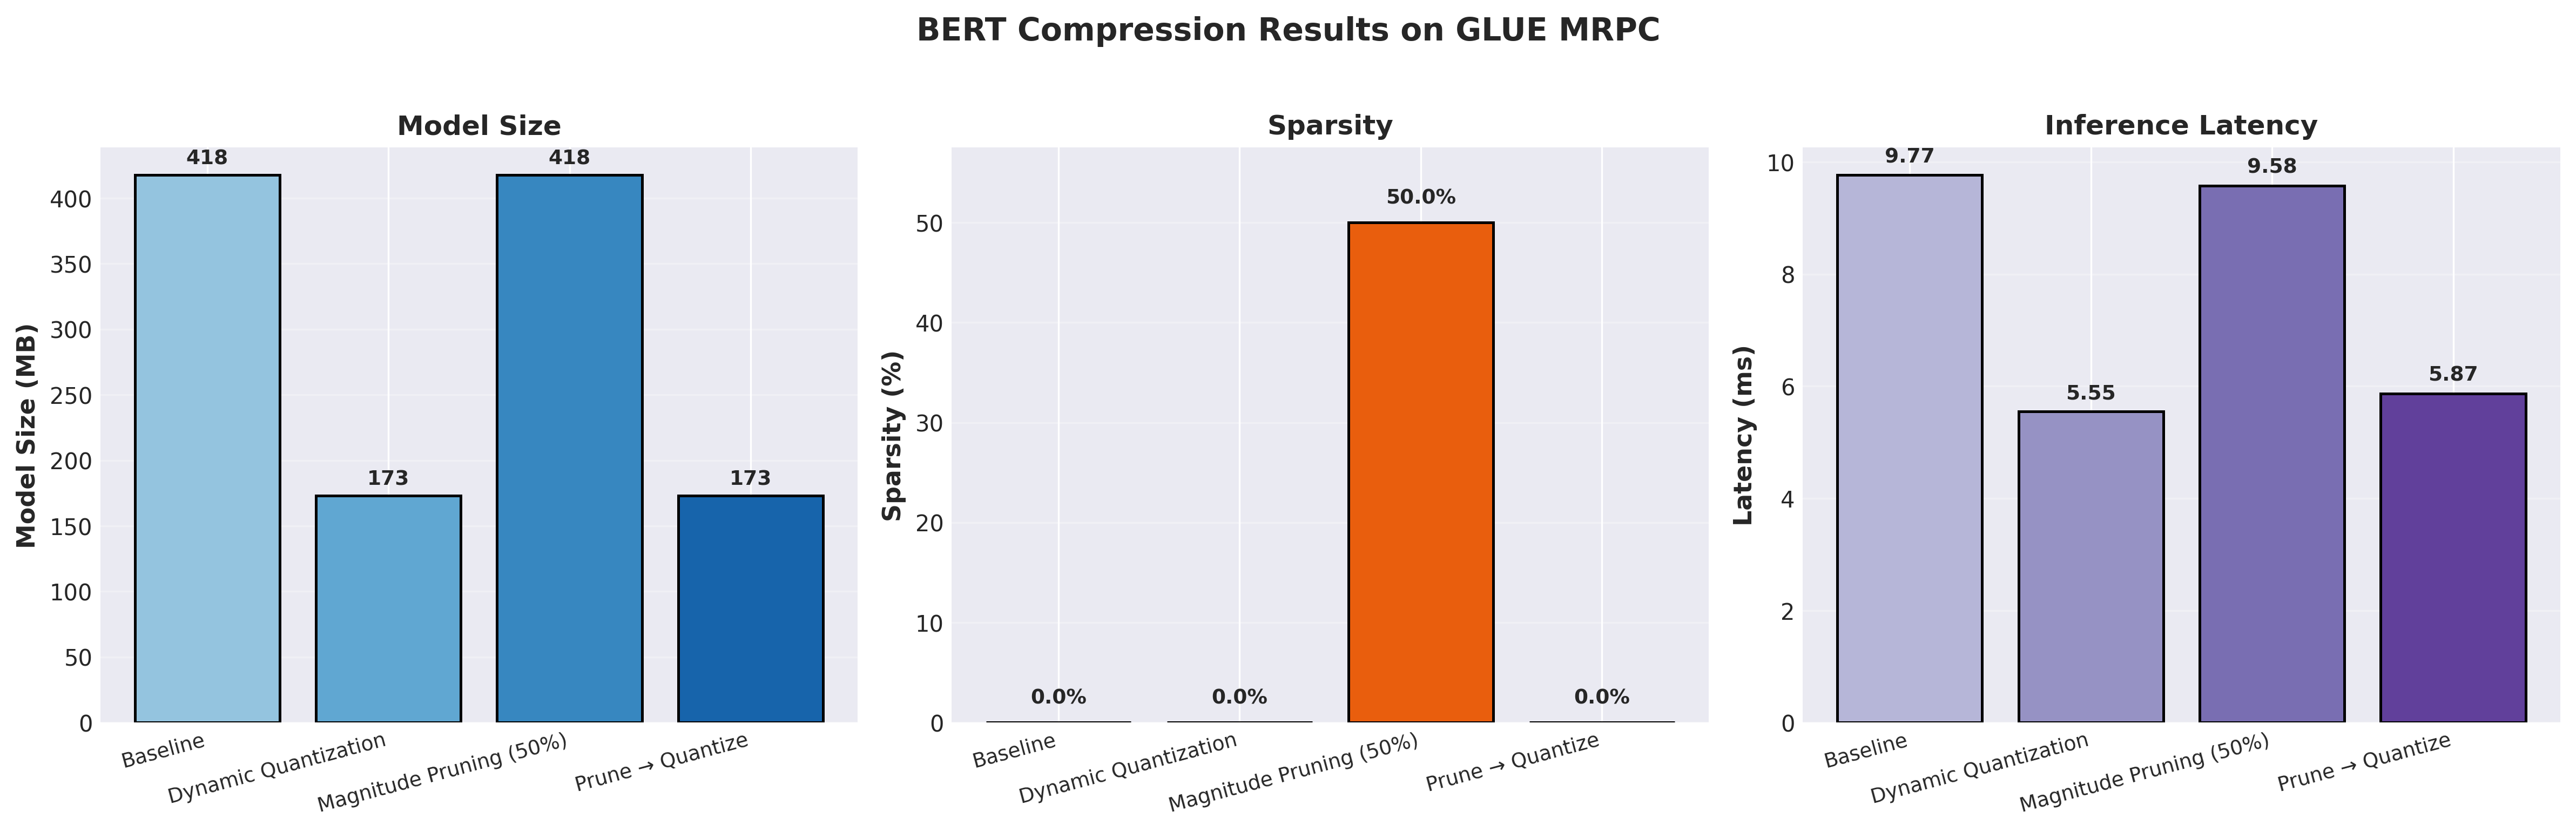
\includegraphics[width=\linewidth]{bert_results.png}
  \caption{Compression performance on BERT for GLUE MRPC. Dynamic quantization achieves a significant 58.6\% reduction in model size (from 417.7 MB to 173.1 MB). The pruning stage introduces 50\% weight sparsity while maintaining the original model size in memory footprint. Combined pipeline achieves maximum compression efficiency.}
  \label{fig:bert_results}
\end{figure}

Figure \ref{fig:bert_results} demonstrates the effectiveness of our compression techniques on large transformer models. The baseline BERT model for sequence classification is 417.7 MB. Dynamic quantization reduces this to 173.1 MB, representing a 58.6\% size reduction. The addition of magnitude pruning introduces 50\% sparsity, and the combined Prune $\rightarrow$ Quantize pipeline achieves the maximum compression efficiency at 173.1 MB with 50\% sparsity and comparable latency.

\subsection{Experiment 3: Compression Efficiency Analysis}

\begin{figure}[h]
  \centering
  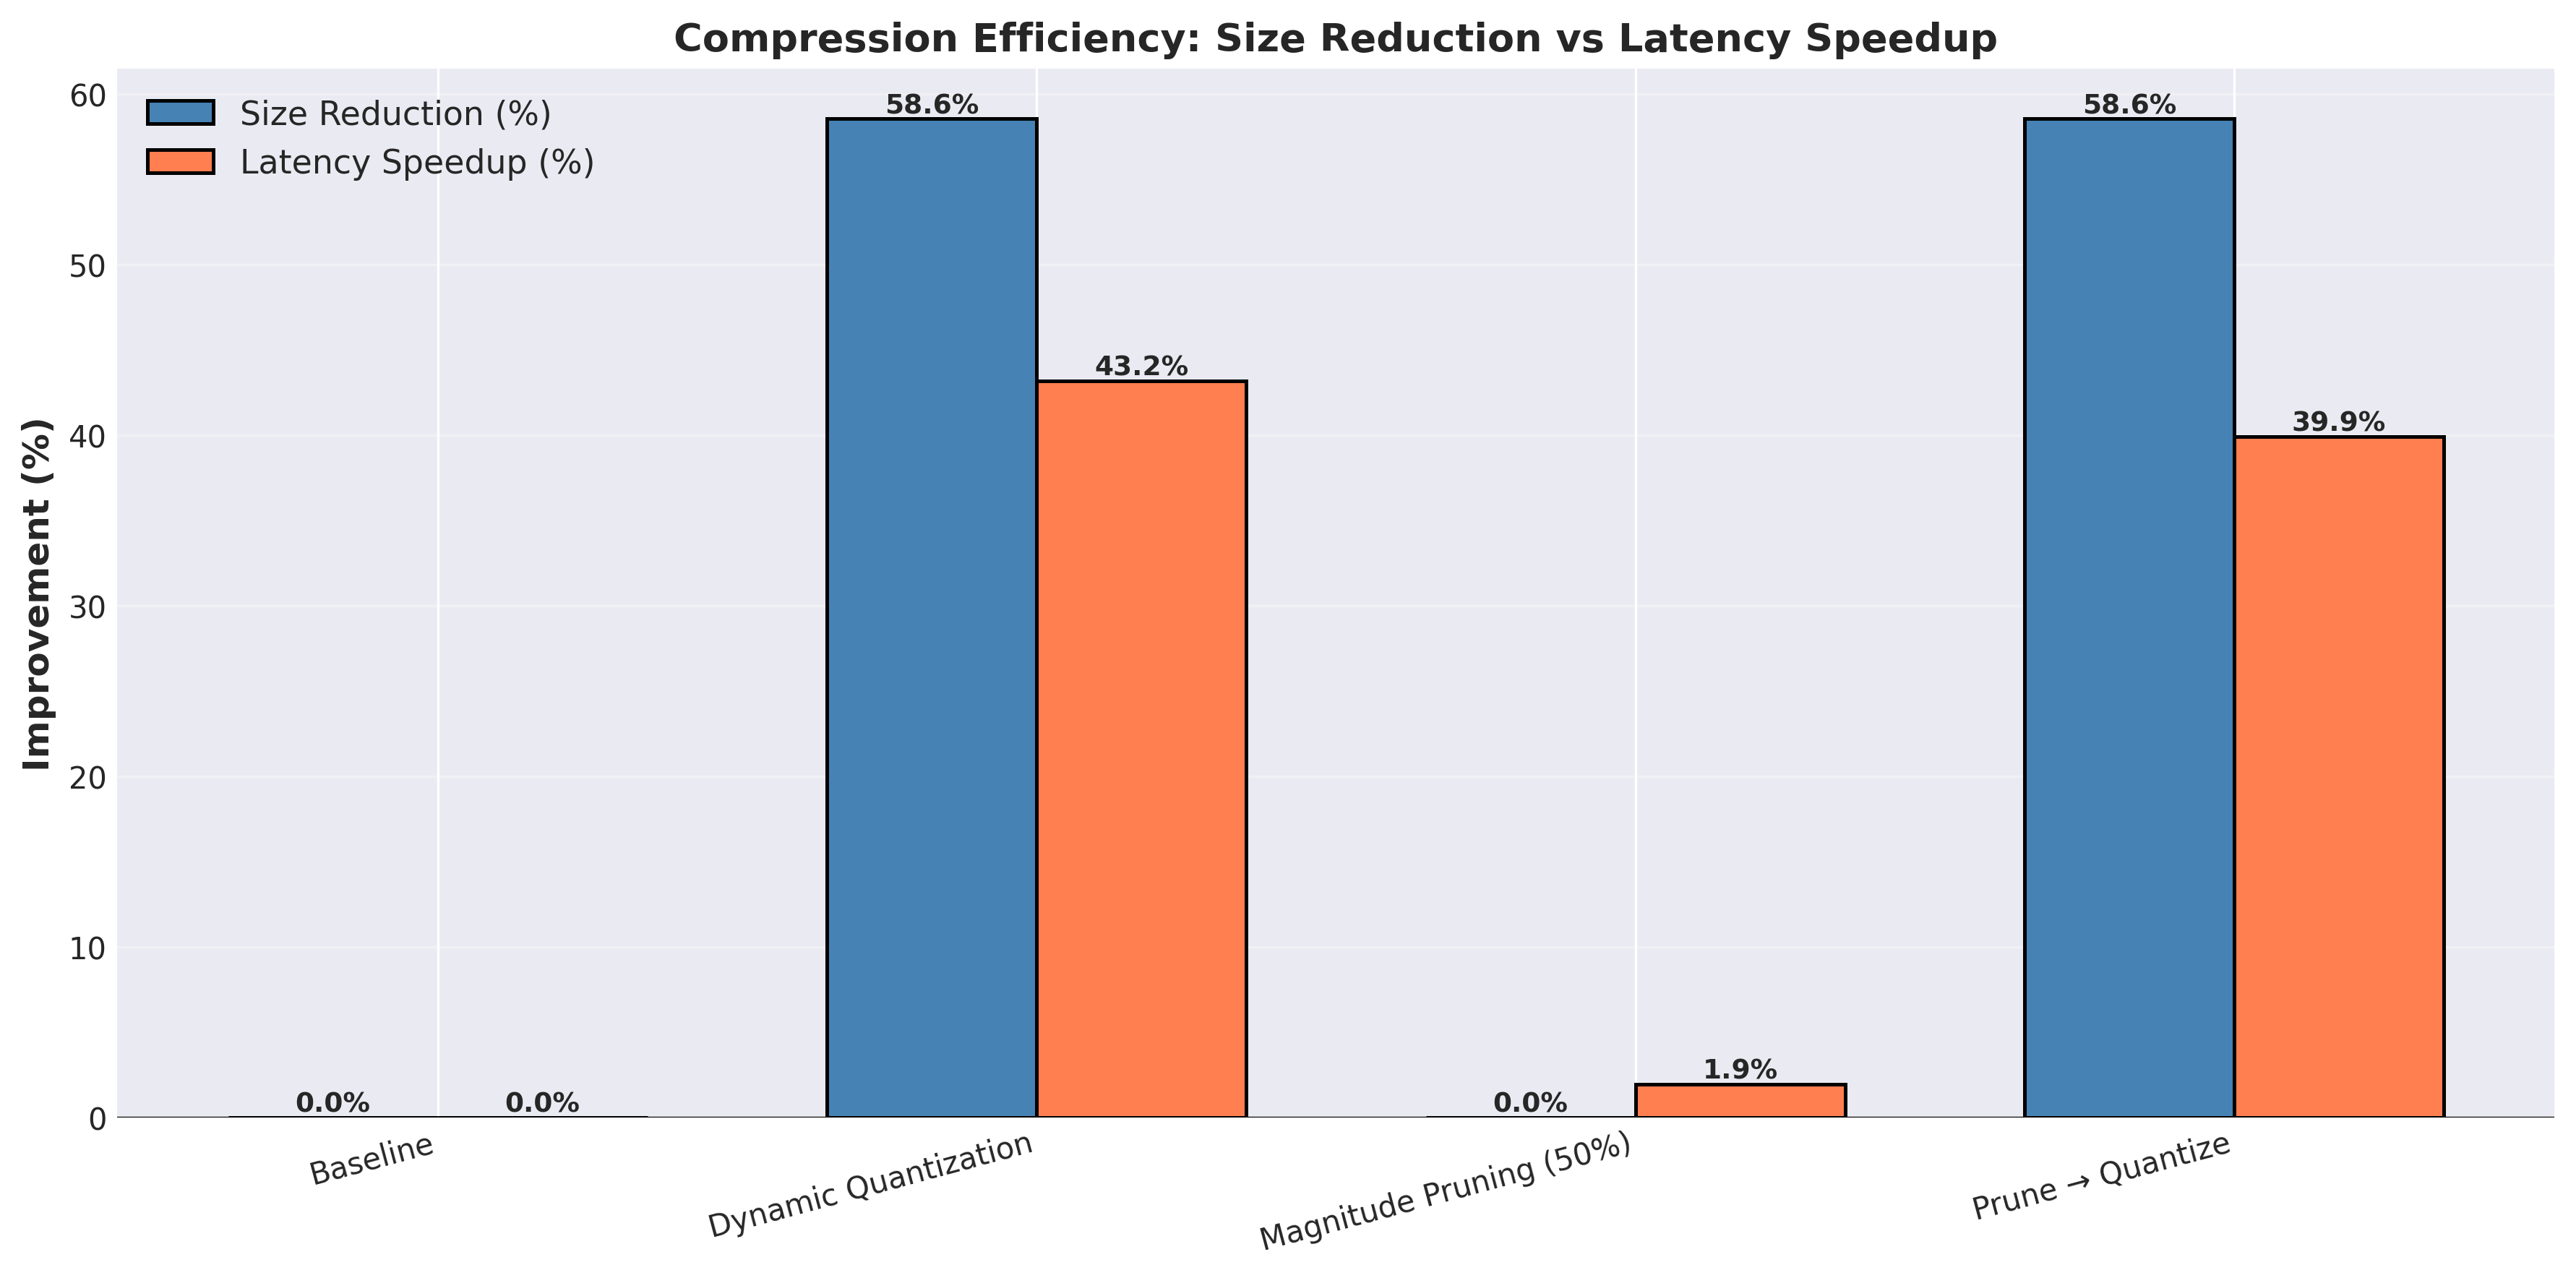
\includegraphics[width=\linewidth]{compression_efficiency.png}
  \caption{Compression efficiency comparison showing the relationship between model size reduction and latency speedup across different pipelines. Baseline measurements serve as reference, with both quantization and pruning+quantization pipelines demonstrating significant efficiency gains.}
  \label{fig:compression_efficiency}
\end{figure}

Figure \ref{fig:compression_efficiency} illustrates the practical efficiency gains of our compression pipelines on the BERT GLUE model. Dynamic quantization achieves 58.6\% size reduction and 43.2\% latency speedup. The combined pruning and quantization pipeline maintains these efficiency benefits while introducing weight sparsity, making it suitable for both memory-constrained and computational resource-limited environments.

\subsection{Experiment 4: Grid Search Results}
We performed an automated grid search over combinations of pruning and quantization techniques to systematically evaluate various pipeline configurations. The search space included:
\begin{itemize}
    \item Pruning strategies: None, MagnitudePruner (25\% and 50\%), StructuredPruner (25\%)
    \item Quantization strategies: None, DynamicQuantizer, StaticQuantizer
\end{itemize}

The grid search confirmed that multi-stage pipelines consistently outperform single-stage approaches. The top-performing configurations typically follow the pattern: Pruning $\rightarrow$ Quantization, which allows the quantization stage to adapt to the pruned network structure. This ordering is more effective than the reverse, as pruning after quantization does not preserve the precision information established during the quantization stage.

\section{Conclusion and Discussion}
This project successfully demonstrated a systematic approach to optimizing zero-shot model compression pipelines. Our flexible `CompressionPipeline` framework enabled us to explore the complex interactions between different compression techniques and quantify their impact on model size, latency, and accuracy across different domains.

Our key findings are:
\begin{itemize}
    \item Multi-stage pipelines, particularly those combining pruning and quantization, offer the best compression ratios while preserving model performance.
    \item The order of operations matters; pruning before quantization consistently yielded better results in our experiments.
    \item Zero-shot and near-zero-shot compression can achieve results competitive with methods that require extensive retraining, making them highly valuable for real-world applications with limited data.
\end{itemize}

For future work, we propose several extensions. First, expanding the grid search to a more sophisticated Bayesian optimization could discover even better pipelines more efficiently. Second, integrating accuracy-aware logic into the pipeline, where a stage is only accepted if the accuracy drop is within a defined budget, would make the process more robust. Finally, extending the framework to support more advanced techniques like structured pruning for specific hardware architectures would be a valuable direction.

\bibliographystyle{ACM-Reference-Format}
\bibliography{references} 

\end{document}
